\documentclass[UTF8,a4paper,11pt]{ctexart}

% ============ 宏包 ============
\usepackage{geometry}
\geometry{left=2.7cm,right=2.7cm,top=2.6cm,bottom=2.4cm,headsep=0.8cm,footskip=0.9cm}
\usepackage{graphicx}
\graphicspath{{img/}}
\usepackage{booktabs,tabularx,array,longtable,multirow}
\usepackage{xcolor}
\usepackage{caption}
\usepackage{enumitem}
\usepackage{fancyhdr}
\usepackage{titlesec}
\usepackage[hidelinks]{hyperref}
\hypersetup{pdftitle={实验三 软件实现与构建：校园二手交易系统},pdfauthor={黄毅 241220107},pdfsubject={软件工程实验三},pdfkeywords={Python, 软件实现, pylint, pytest, Git, 校园二手交易}}
\usepackage{amsmath}
\usepackage{listings}
\usepackage{fontspec}
\setmonofont{Consolas}
\setCJKmonofont{SimSun}
\setcounter{tocdepth}{2}

% ============ 代码与终端输出样式 ============
\definecolor{listbg}{HTML}{F7F8FA}
\definecolor{listframe}{HTML}{C9D2DB}
\lstset{
  basicstyle=\ttfamily\scriptsize,
  columns=fixed,
  basewidth=0.5em,
  keepspaces=true,
  breaklines=true,
  breakatwhitespace=false,
  frame=single,
  rulecolor=\color{listframe},
  backgroundcolor=\color{listbg},
  showstringspaces=false,
  tabsize=4,
  xleftmargin=0.6em,
  xrightmargin=0.6em,
  aboveskip=0.6em,
  belowskip=0.4em,
}

% ============ 样式 ============
\linespread{1.28}
\emergencystretch=4em
\setlength{\parskip}{0.25em}
\setlength{\topsep}{3pt}
\setlength{\partopsep}{1pt}
\counterwithin*{figure}{section}
\counterwithin*{table}{section}
\renewcommand{\thefigure}{\thesection-\arabic{figure}}
\renewcommand{\thetable}{\thesection-\arabic{table}}

\setcounter{topnumber}{3}
\setcounter{bottomnumber}{1}
\setcounter{totalnumber}{5}
\renewcommand{\topfraction}{0.92}
\renewcommand{\bottomfraction}{0.7}
\renewcommand{\textfraction}{0.06}
\renewcommand{\floatpagefraction}{0.75}
\captionsetup{font={small,stretch=1.1},labelsep=quad,justification=centering}
\captionsetup[table]{skip=4pt}

\ctexset{
  section={format=\zihao{3}\heiti\bfseries, beforeskip=14pt, afterskip=10pt, name={,},number=\arabic{section}},
  subsection={format=\zihao{4}\heiti\bfseries, beforeskip=10pt, afterskip=7pt},
  subsubsection={format=\zihao{-4}\heiti\bfseries, beforeskip=8pt, afterskip=5pt},
}
\renewcommand{\thesection}{\arabic{section}}
\renewcommand{\thesubsection}{\thesection.\arabic{subsection}}
\renewcommand{\thesubsubsection}{\thesubsection.\arabic{subsubsection}}

\pagestyle{fancy}
\fancyhf{}
\fancyhead[L]{\zihao{-5}\songti 软件工程 · 实验三：软件实现与构建}
\fancyhead[R]{\zihao{-5}\songti 校园二手交易系统}
\fancyfoot[C]{\zihao{-5}\thepage}
\renewcommand{\headrulewidth}{0.4pt}
\renewcommand{\footrulewidth}{0pt}

\newcolumntype{Y}{>{\raggedright\arraybackslash}X}
\newcolumntype{L}[1]{>{\raggedright\arraybackslash}p{#1}}
\newcommand{\tabfont}{\zihao{5}}
\newcommand{\figref}[1]{图~\ref{#1}}
\newcommand{\tabref}[1]{表~\ref{#1}}
% \hspace{0pt} 在行内代码前后各加一个零宽断点，避免长标识符把行撑出边界
\newcommand{\code}[1]{\hspace{0pt}\texttt{#1}\hspace{0pt}}

\begin{document}
\zihao{-4}

% ================= 封面 =================
\definecolor{accent}{HTML}{0E9F6E}
\definecolor{inkc}{HTML}{16202B}
\begin{titlepage}
\thispagestyle{empty}
\begin{center}
\vspace*{1.6cm}

{\zihao{-3}\heiti 软\quad 件\quad 工\quad 程}\\[6pt]
{\color{accent}\rule{3.6cm}{0.9pt}}

\vspace{1.5cm}
{\zihao{-1}\heiti\bfseries 实验三：软件实现与构建}

\vspace{0.9cm}
{\zihao{4}\kaishu 校园二手交易系统的编码实现、静态检查与仓库托管}

\vspace{2.2cm}

\renewcommand{\arraystretch}{1.75}
{\zihao{4}\songti
\begin{tabular}{r@{\hspace{0.7em}}l}
\toprule
课程名称 & 软件工程 \\
项目名称 & 校园二手交易系统（CampusTrade）\\
学\qquad 号 & 241220107 \\
姓\qquad 名 & 黄\quad 毅 \\
学\qquad 院 & 计算机科学与技术学院 \\
专\qquad 业 & 计算机科学与技术 \\
任课教师 & 王\quad 豫 \\
完成日期 & 2026 年 11 月 \\
\bottomrule
\end{tabular}
}

\vfill
{\zihao{5}\songti\color{gray}
依据实验一 19 条需求与实验二 6 张 UML 图实现\\
Python 3，22 个源文件、3311 行，73 个单元测试\\
远程仓库 APY-tech/Software-Engineering}
\end{center}
\end{titlepage}

% ================= 目录 =================
\pagenumbering{roman}
\setcounter{page}{1}
\setcounter{tocdepth}{1}
\tableofcontents
\clearpage
\pagenumbering{arabic}
\setcounter{page}{1}

\section{实现概述}

\subsection{实现目标与技术选型}

本次实验要把实验二的设计变成可编译、可运行、可测试的软件：8 个组件、10 个领域类、7 个商品状态、19 条需求（15 条功能、3 条非功能、1 条待确认）。语言选 \textbf{Python 3.13}，只使用标准库，运行时不需要安装任何第三方包；界面采用\textbf{命令行菜单}，没有做图形界面。

选型理由有三条。第一，本系统的难点不在界面而在规则：同一商品至多一条有效预约、审核期间商品仍可被预约、已发布商品改内容要"前台显示旧信息、后台审新内容"。这些规则的组合爆炸靠人工枚举容易漏，用 Python 写测试验证最省力。第二，后续实验要对程序做静态分析与测试，Python 生态里的 \code{pylint}、\allowbreak \code{pytest} 可以直接对被测代码做度量，不需要额外搭桩。第三，只用标准库可以保证在机房机器和自备机器上结果一致，避免环境差异带来的"在我这里能跑"。

不做图形界面是权衡后的决定：实验二已给出 10 张界面稿，但本次的重点是规则正确性，控制台界面用 \code{Shell} 的 30 个菜单项把全部用例走通，界面层与业务层完全分离，将来换成 Tkinter 或 Web 只需替换 \code{campustrade/cli} 目录，服务层一行不改。代价是演示时看不到视觉反馈，这一点在第 7 节作为不足记录。

\subsection{总体结构}

代码分五层，依赖方向单向向下，界面层不允许直接碰仓储（\tabref{tab:layer}）。

\begin{table}[htbp]
\centering
\caption{代码分层与职责（行数含空行与注释）}\label{tab:layer}
\zihao{-5}
\renewcommand{\arraystretch}{1.18}
\begin{tabularx}{\textwidth}{@{}L{2.05cm}L{4.5cm}YL{1.35cm}@{}}
\toprule
层 & 文件 & 职责 & 行数 \\
\midrule
领域模型 & \code{models.py}、\allowbreak \code{errors.py}、\allowbreak \code{state.py} & 实体、枚举、值对象、异常层次、状态迁移表 & 513 \\
基础设施 & \code{storage.py}、\allowbreak \code{security.py} & 内存表 + JSON 快照、口令散列与会话令牌 & 305 \\
服务层 & \code{services/}（9 个文件） & 认证、商品、审核、交易、举报、统计、日志与通知 & 1343 \\
界面层 & \code{cli/shell.py}、\allowbreak \code{cli/tables.py} & 菜单、输入校验、中文宽度对齐的表格 & 602 \\
装配与入口 & \code{context.py}、\allowbreak \code{seed.py}、\allowbreak \code{demo.py}、\allowbreak \code{run.py} & 依赖装配、演示数据、端到端脚本、参数解析 & 548 \\
\midrule
合计 & 22 个源文件 & —— & 3311 \\
\bottomrule
\end{tabularx}
\end{table}

装配集中在 \code{context.py} 的 \code{build\_application()}：先建仓储与日志，再建认证，最后建六个业务服务。依赖顺序写在一处，服务之间就不会互相 \code{import} 造成循环，测试里也能一行拿到整套服务。

\subsection{五个关键实现决定}

\begin{enumerate}[leftmargin=1.6em,itemsep=2pt,topsep=3pt]
\item \textbf{状态只有一处可写}。商品状态不对外暴露 setter，所有迁移都走 \code{apply\_status()}，它先查迁移表再赋值并递增版本号。7 个状态之间的 9 条合法迁移与实验二状态图一一对应，非法迁移抛 \code{Conflict}，错误信息里带当前状态和版本。
\item \textbf{权限判断跟着服务走，不跟着界面走}。每个面向界面的方法第一个参数都是会话令牌，方法内部换成 \code{User} 再判断角色与归属。界面层因此不可能"忘记"校验，测试也能直接拿不同角色的令牌调同一个方法。
\item \textbf{持久化用整库快照 + 原子替换}。写临时文件后 \code{os.replace()}，即使进程中途被杀也不会留下半截 JSON。课程作业的数据量在千条级，这个方案比引入数据库省事，也便于人工查看数据。
\item \textbf{并发只在必要处加锁}。仓储持有一把可重入锁，\code{TradeService.reserve()} 与 \code{cancel/confirm} 在临界区内完成"查重—校验—写入"，其余操作不加锁。锁的范围就是"同一商品至多一条有效预约"这条不变式需要保护的范围。
\item \textbf{异常分层}。\code{DomainError} 之下分五类，各管一件事：入参不合法 \code{ValidationError}、未登录或过期 \code{AuthError}、越权 \code{PermissionDenied}、目标不存在 \code{NotFound}、与当前状态冲突 \code{Conflict}。界面层只在一个地方捕获并打印，服务层不返回错误码、不打印日志。
\end{enumerate}

\subsection{与实验二组件的对应}

实验二把系统划成 8 个模块（M1--M8），实现时按依赖方向落成 7 个服务加 1 个横切模块（\tabref{tab:module}）。分量基本对齐，只有两处合并：M4 查询并入商品服务（查询的条件就是商品属性，拆开会出现两个服务同时读 \code{Item}）、M8 公共支撑拆成 \code{storage} 与 \code{journal} 两部分（一个管持久化、一个管日志与通知）。

\begin{table}[htbp]
\centering
\caption{实验二组件到实验三模块的映射}\label{tab:module}
\zihao{-5}
\renewcommand{\arraystretch}{1.15}
\begin{tabularx}{\textwidth}{@{}L{1.5cm}L{3.4cm}L{3.6cm}Y@{}}
\toprule
组件 & 实验二职责 & 实现位置 & 说明 \\
\midrule
M1 & 用户与权限 & \code{services/auth.py} & 注册、登录、会话过期、角色分配 \\
M2 & 商品管理 & \code{services/item.py} & 草稿、修改、送审、下架、分类维护 \\
M3 & 审核 & \code{services/audit.py} & 通过/驳回、审核记录、待审内容原子替换 \\
M4 & 查询 & 并入 M2 & 按关键词、分类、价格、排序过滤 \\
M5 & 交易 & \code{services/trade.py} & 预约、取消、确认、完成、超时自动完成 \\
M6 & 举报治理 & \code{services/moderation.py} & 举报去重、下架/驳回处置 \\
M7 & 日志与统计 & \code{services/journal.py}、\allowbreak \code{stats.py} & 日志只追加、两套统计口径 \\
M8 & 公共支撑 & \code{storage.py}、\allowbreak \code{journal.py} & 快照持久化、通知 \\
\bottomrule
\end{tabularx}
\end{table}

\section{从 UML 图到代码}

每种 UML 元素只对应一种写法，规则先定下，后面逐类翻译即可（\tabref{tab:mapping}）。

\begin{table}[htbp]
\centering
\caption{UML 元素到 Python 构造的转换规则}\label{tab:mapping}
\zihao{-5}
\renewcommand{\arraystretch}{1.2}
\begin{tabularx}{\textwidth}{@{}L{2.5cm}L{4.3cm}Y@{}}
\toprule
UML 元素 & 代码构造 & 处理要点 \\
\midrule
类（实体） & \code{@dataclass} & 字段照抄；主键统一暴露 \code{ident} \\
枚举 & \code{class X(str, Enum)} & 便于 JSON 落盘与按名字解析 \\
关联（1—N） & 外键字段 + 仓储查询 & 不挂对象引用，避免循环引用 \\
组合（Item—ItemRevision） & 独立表 + 按 \code{itemId} 查 & 待审内容能被单独丢弃 \\
操作（方法） & 服务层方法 & 跨聚合读写放服务层 \\
状态图 & 迁移表 + \code{apply\_status} & 每条箭头一个表项 \\
时序图 & 一个方法体 + 锁 & \code{alt} 分支即 \code{if/else} \\
\bottomrule
\end{tabularx}
\end{table}

\subsection{类图}

领域模型（\figref{fig:class}）照实验二类图逐类翻译，10 个实体加 5 个枚举落在 \code{models.py}。实体只保留自身判断，跨实体协作放服务层。\code{ItemRevision} 是组合状态载体：已发布商品被修改时 \code{Item.status} 仍为已发布，新内容暂存于待审记录，审核通过后原子替换。\code{Reservation.requestId} 是幂等键。

\begin{figure}[!htbp]
\centering
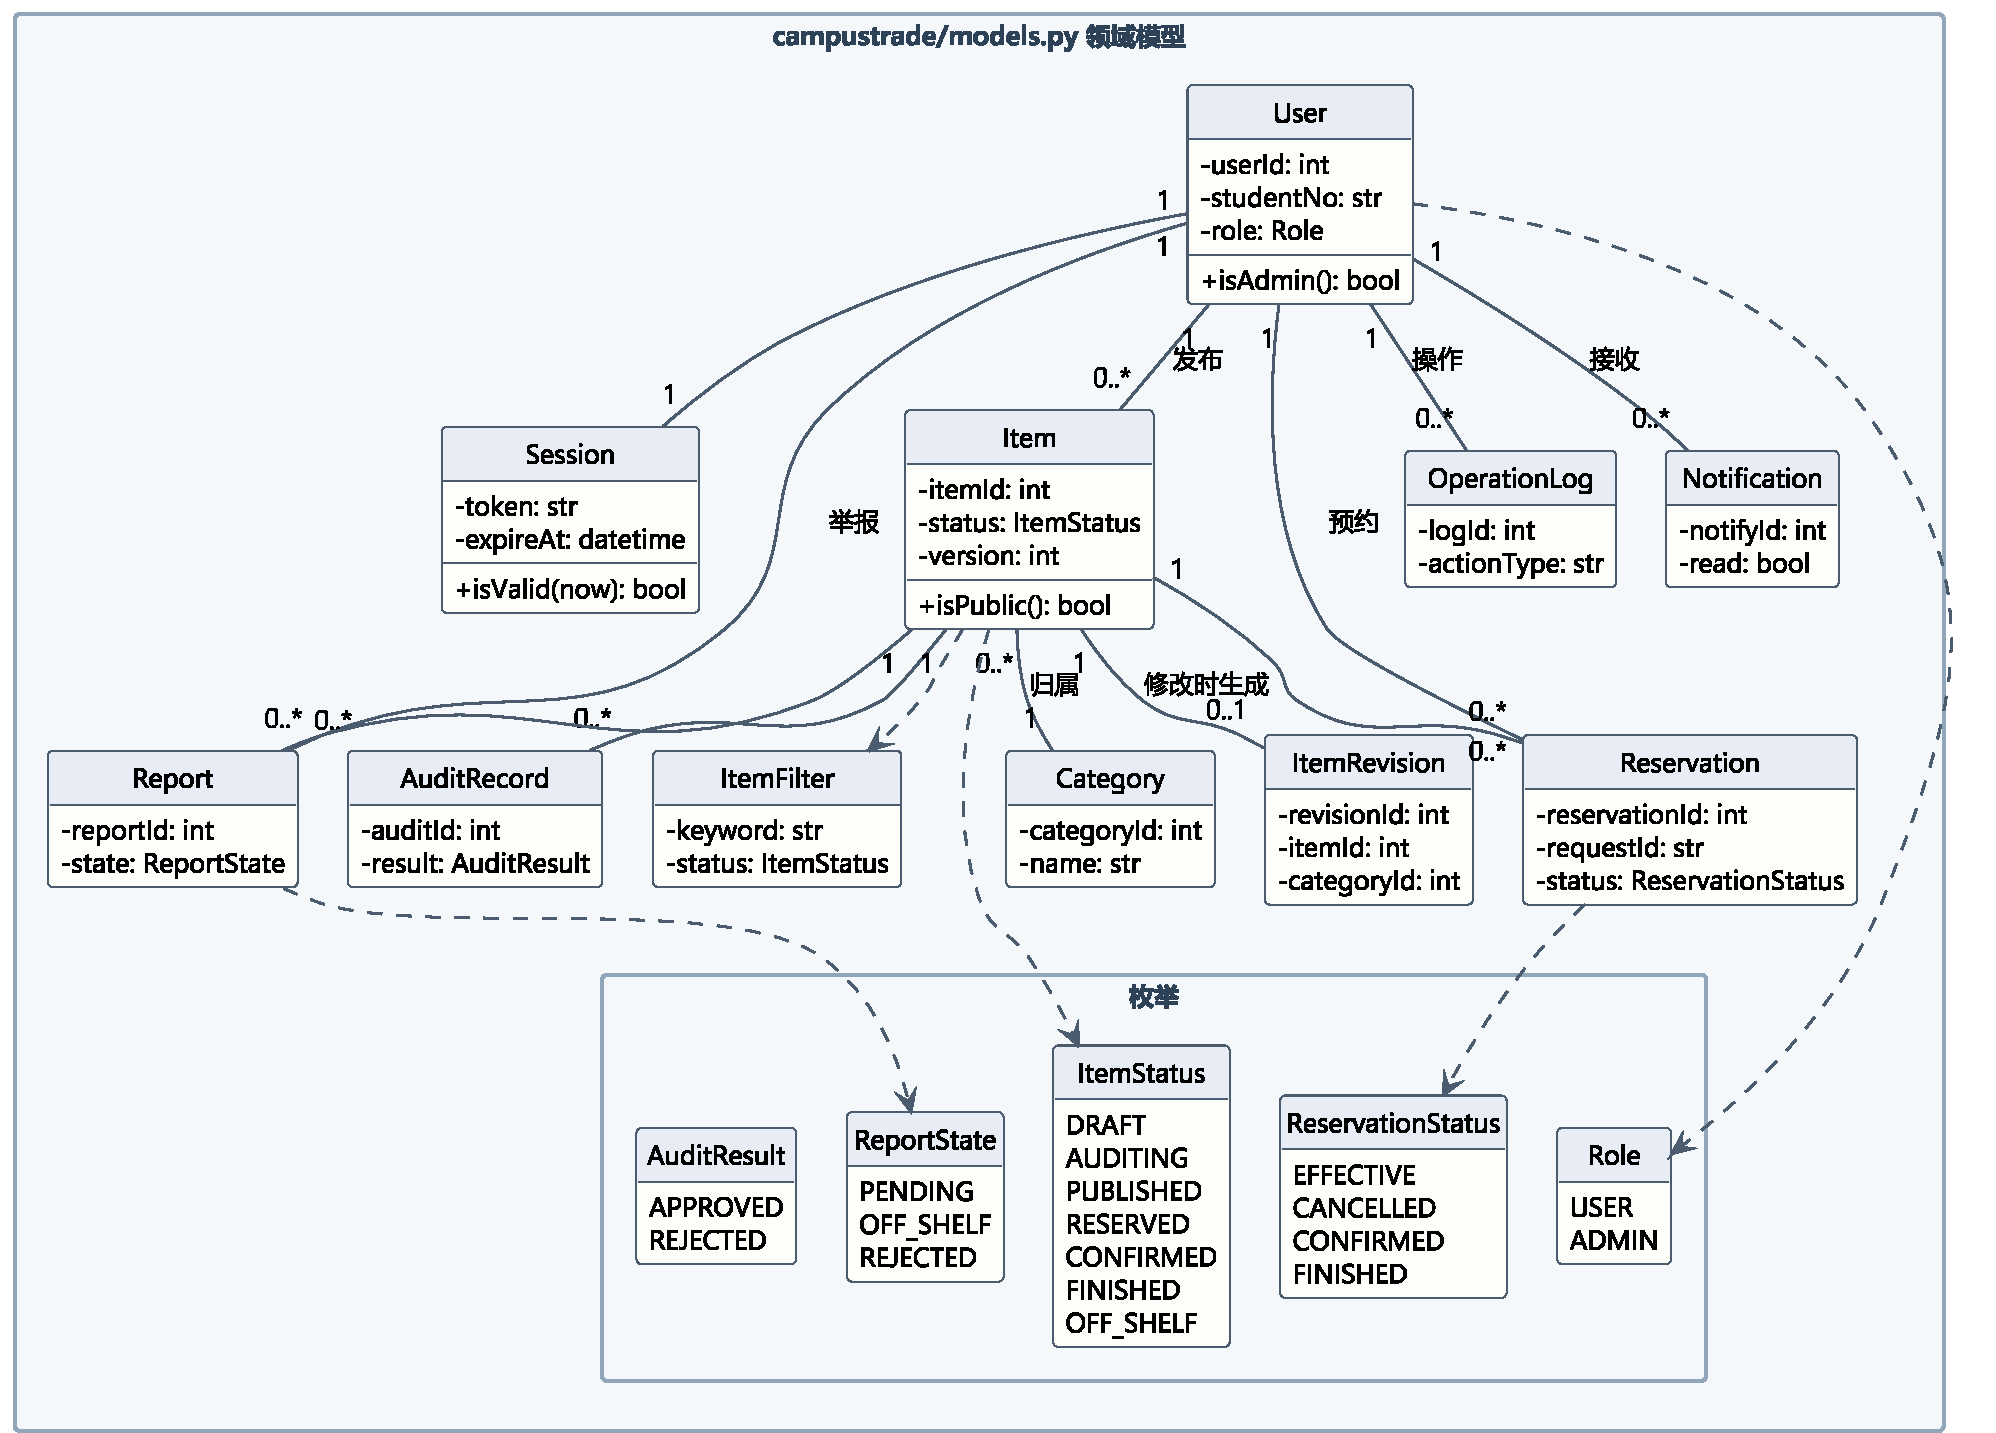
\includegraphics[width=\textwidth]{class.pdf}
\caption{领域模型类图}\label{fig:class}
\end{figure}

服务层与仓储（\figref{fig:service}）是实现期新增：\code{ServiceBase} 收敛令牌换用户与落盘，六个业务服务继承它；\code{Store} 是仓储门面，\code{Table} 是泛型内存表。

\begin{figure}[!htbp]
\centering
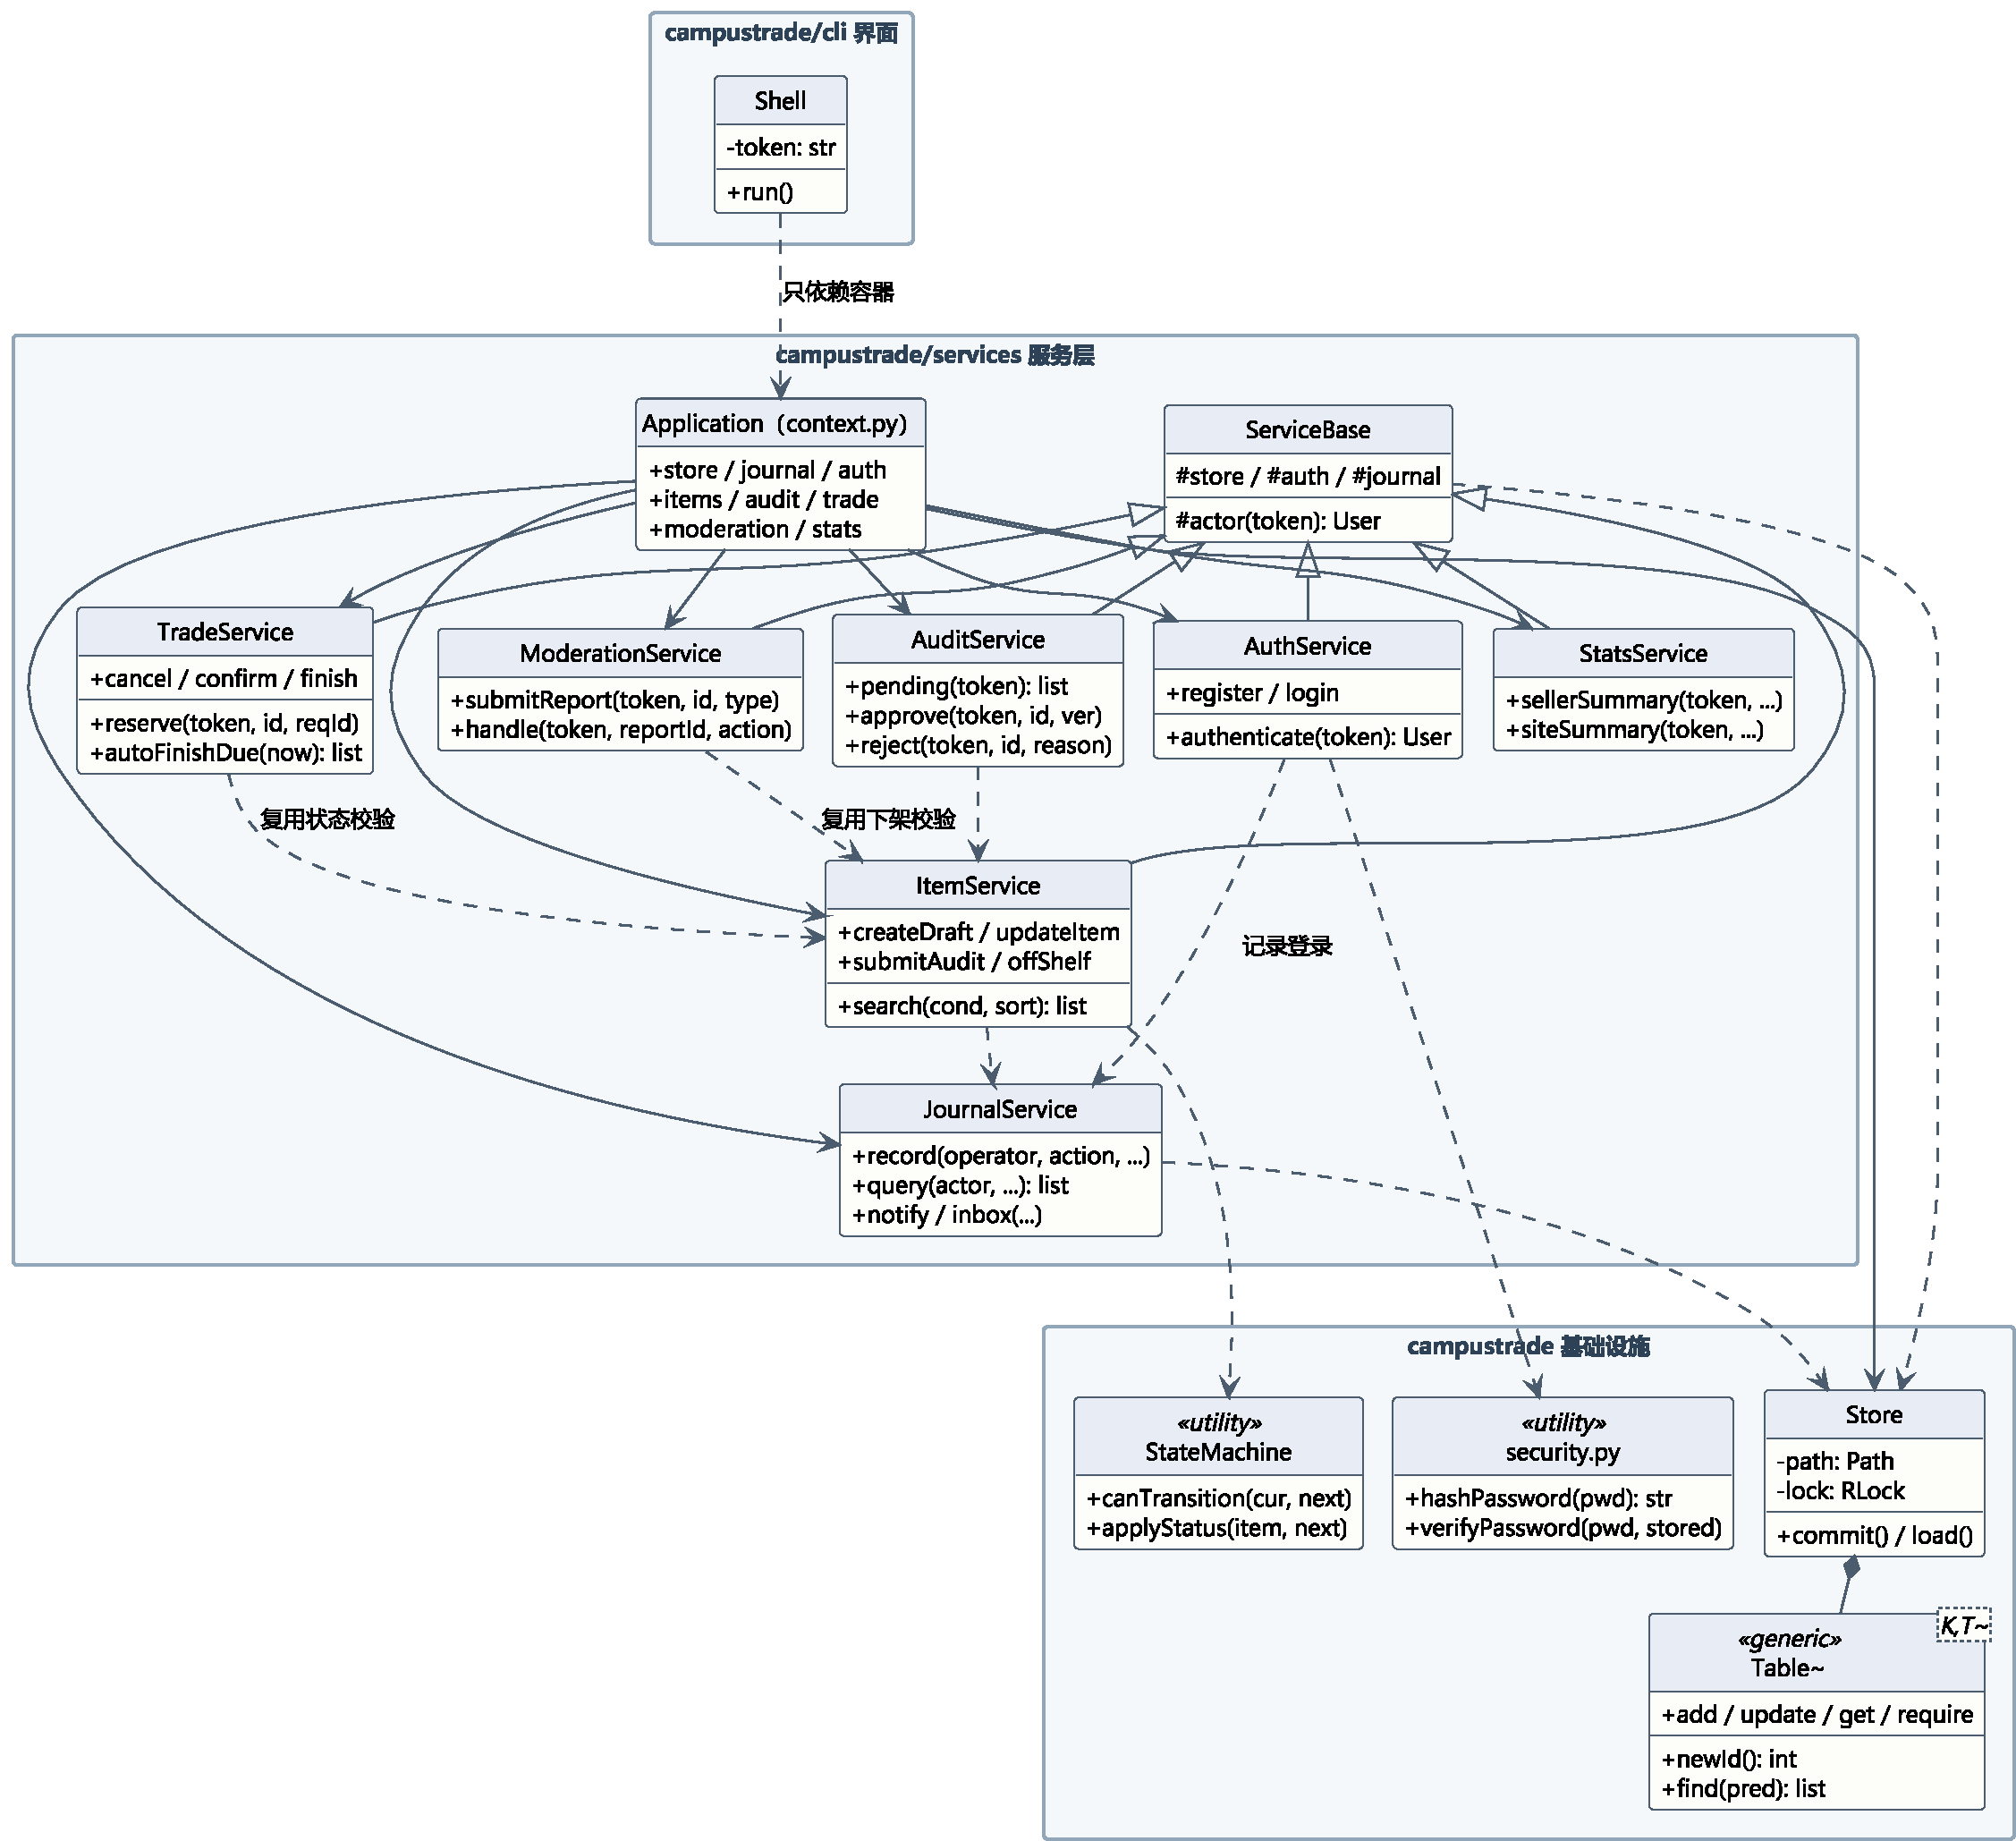
\includegraphics[width=0.82\textwidth]{service.pdf}
\caption{服务层与仓储类图}\label{fig:service}
\end{figure}

实现时对原设计改了三处：一是实体上的业务方法上移到服务层（方法需跨聚合读写，实体会被迫持有仓储引用，事务边界不清）；二是 \code{ItemRevision} 增加 \code{categoryId}（改分类也属修改商品信息，不带分类会导致审核后内容与分类不一致）；三是新增 \code{ServiceBase}、\code{Store}、\code{Table} 三个工程类，收敛重复代码。

\subsection{状态图}

7 个状态、9 条合法迁移写成 \code{state.py} 里的一个字典，\code{apply\_status()} 先校验再赋值并递增 \code{version}（\figref{fig:state}、\tabref{tab:transition}）。非法迁移一律抛 \code{Conflict}。

\begin{figure}[!htbp]
\centering
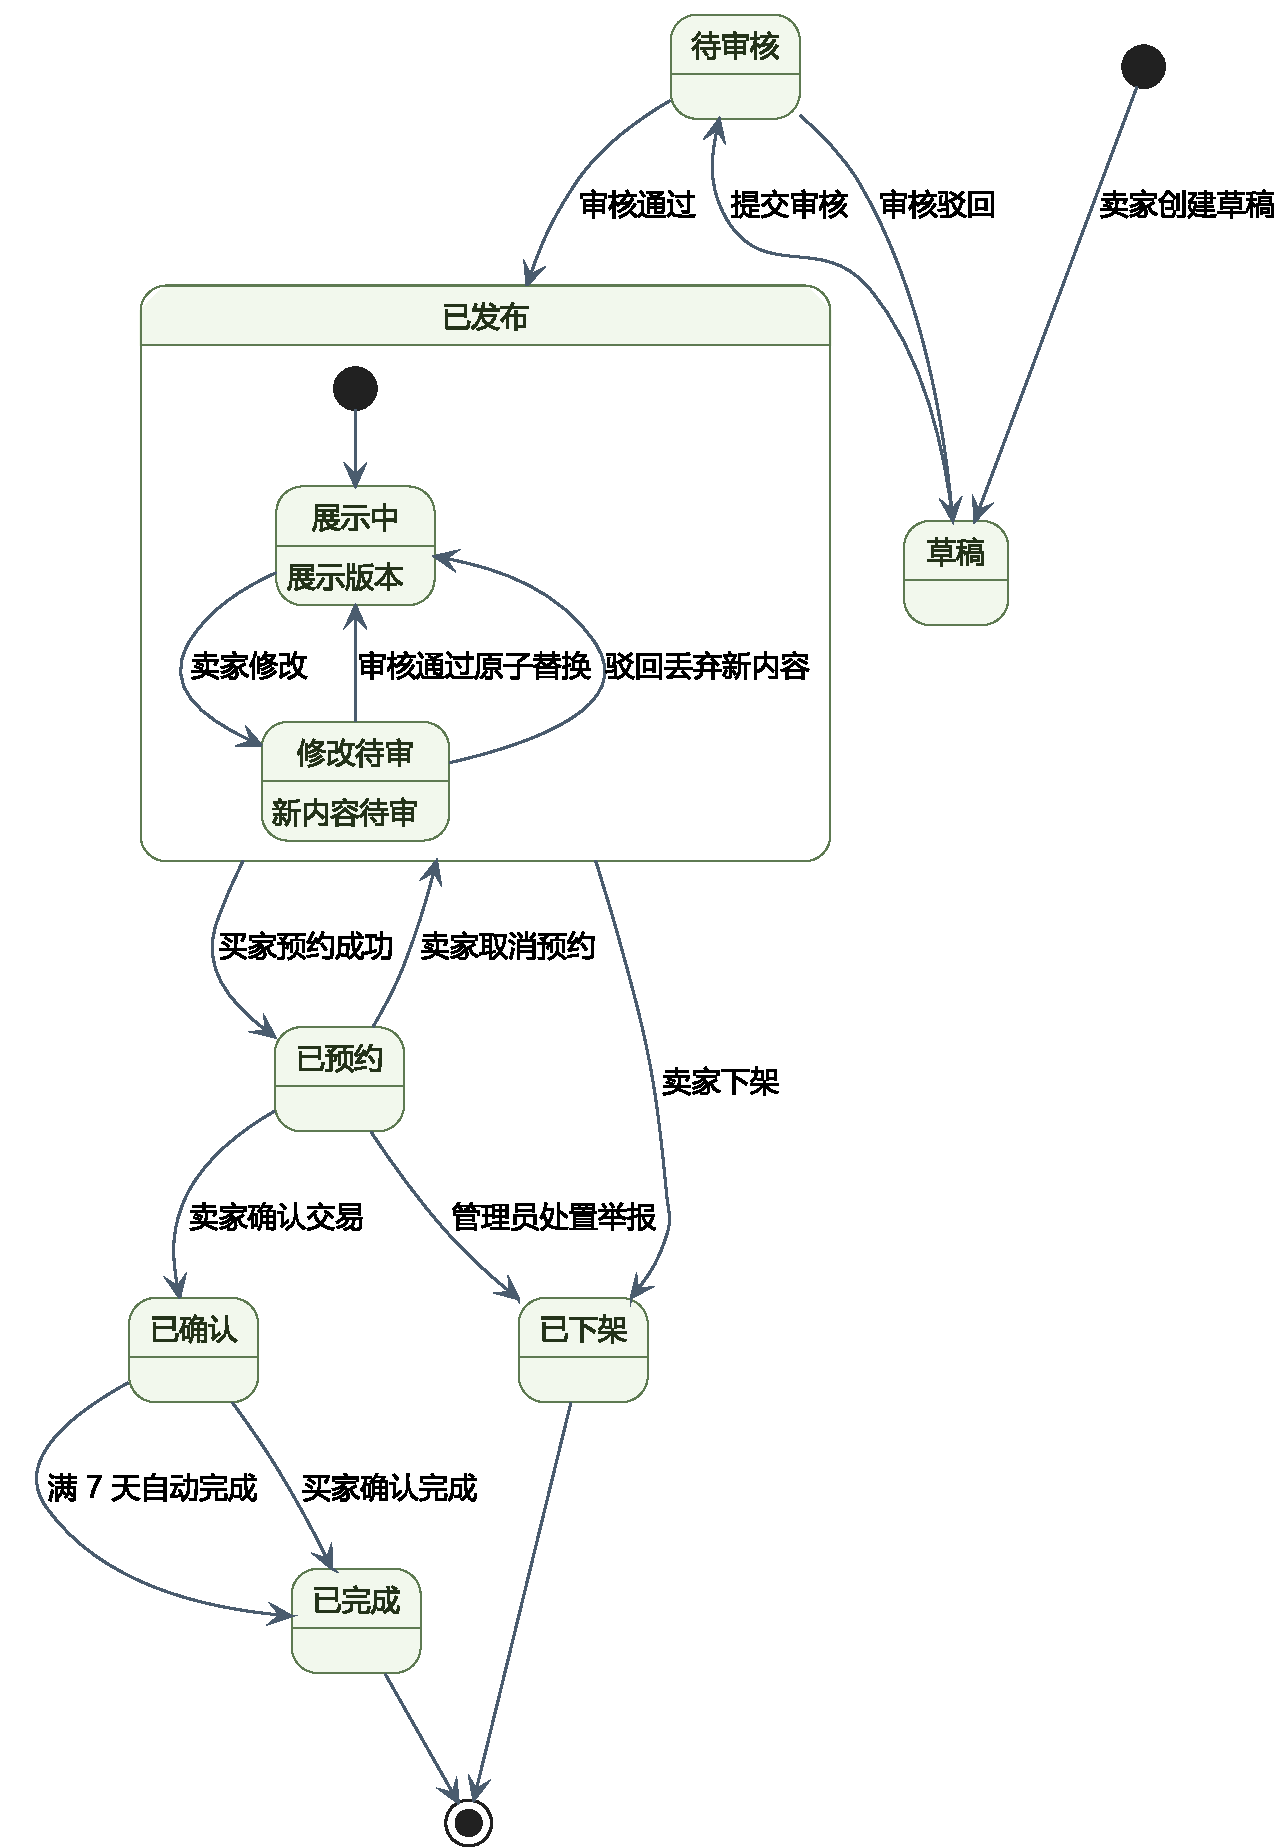
\includegraphics[width=0.29\textwidth]{state.pdf}
\caption{商品状态图}\label{fig:state}
\end{figure}

\begin{table}[htbp]
\centering
\caption{状态迁移与触发动作}\label{tab:transition}
\zihao{-5}
\renewcommand{\arraystretch}{1.15}
\begin{tabularx}{\textwidth}{@{}L{3.3cm}L{4.3cm}Y@{}}
\toprule
迁移 & 触发方法 & 附加校验 \\
\midrule
草稿 $\to$ 待审核 & \code{ItemService.submit\_audit} & 必填字段；仅本人 \\
待审核 $\to$ 已发布 & \code{AuditService.approve} & 仅管理员；版本比对 \\
待审核 $\to$ 草稿 & \code{AuditService.reject} & 必填驳回原因 \\
已发布 $\to$ 已预约 & \code{TradeService.reserve} & 锁内查重；幂等键 \\
已预约 $\to$ 已发布 & \code{TradeService.cancel} & 仅卖家 \\
已预约 $\to$ 已确认 & \code{TradeService.confirm} & 仅卖家 \\
已确认 $\to$ 已完成 & \code{TradeService.finish} & 仅预约买家；满 7 天自动完成 \\
已发布 $\to$ 已下架 & \code{ItemService.off\_shelf} & 仅本人或管理员 \\
已下架 $\to$ 已发布 & \code{ItemService.restore} & 仅管理员 \\
\bottomrule
\end{tabularx}
\end{table}

\subsection{时序图}

预约流程按\figref{fig:seq}逐条翻译，\code{alt} 分支对应 \code{raise}，\code{with store.lock} 对应临界区。查重放在最前，重发请求此时商品已是已预约，若先校验状态会把重发误判为冲突。

\begin{figure}[!htbp]
\centering
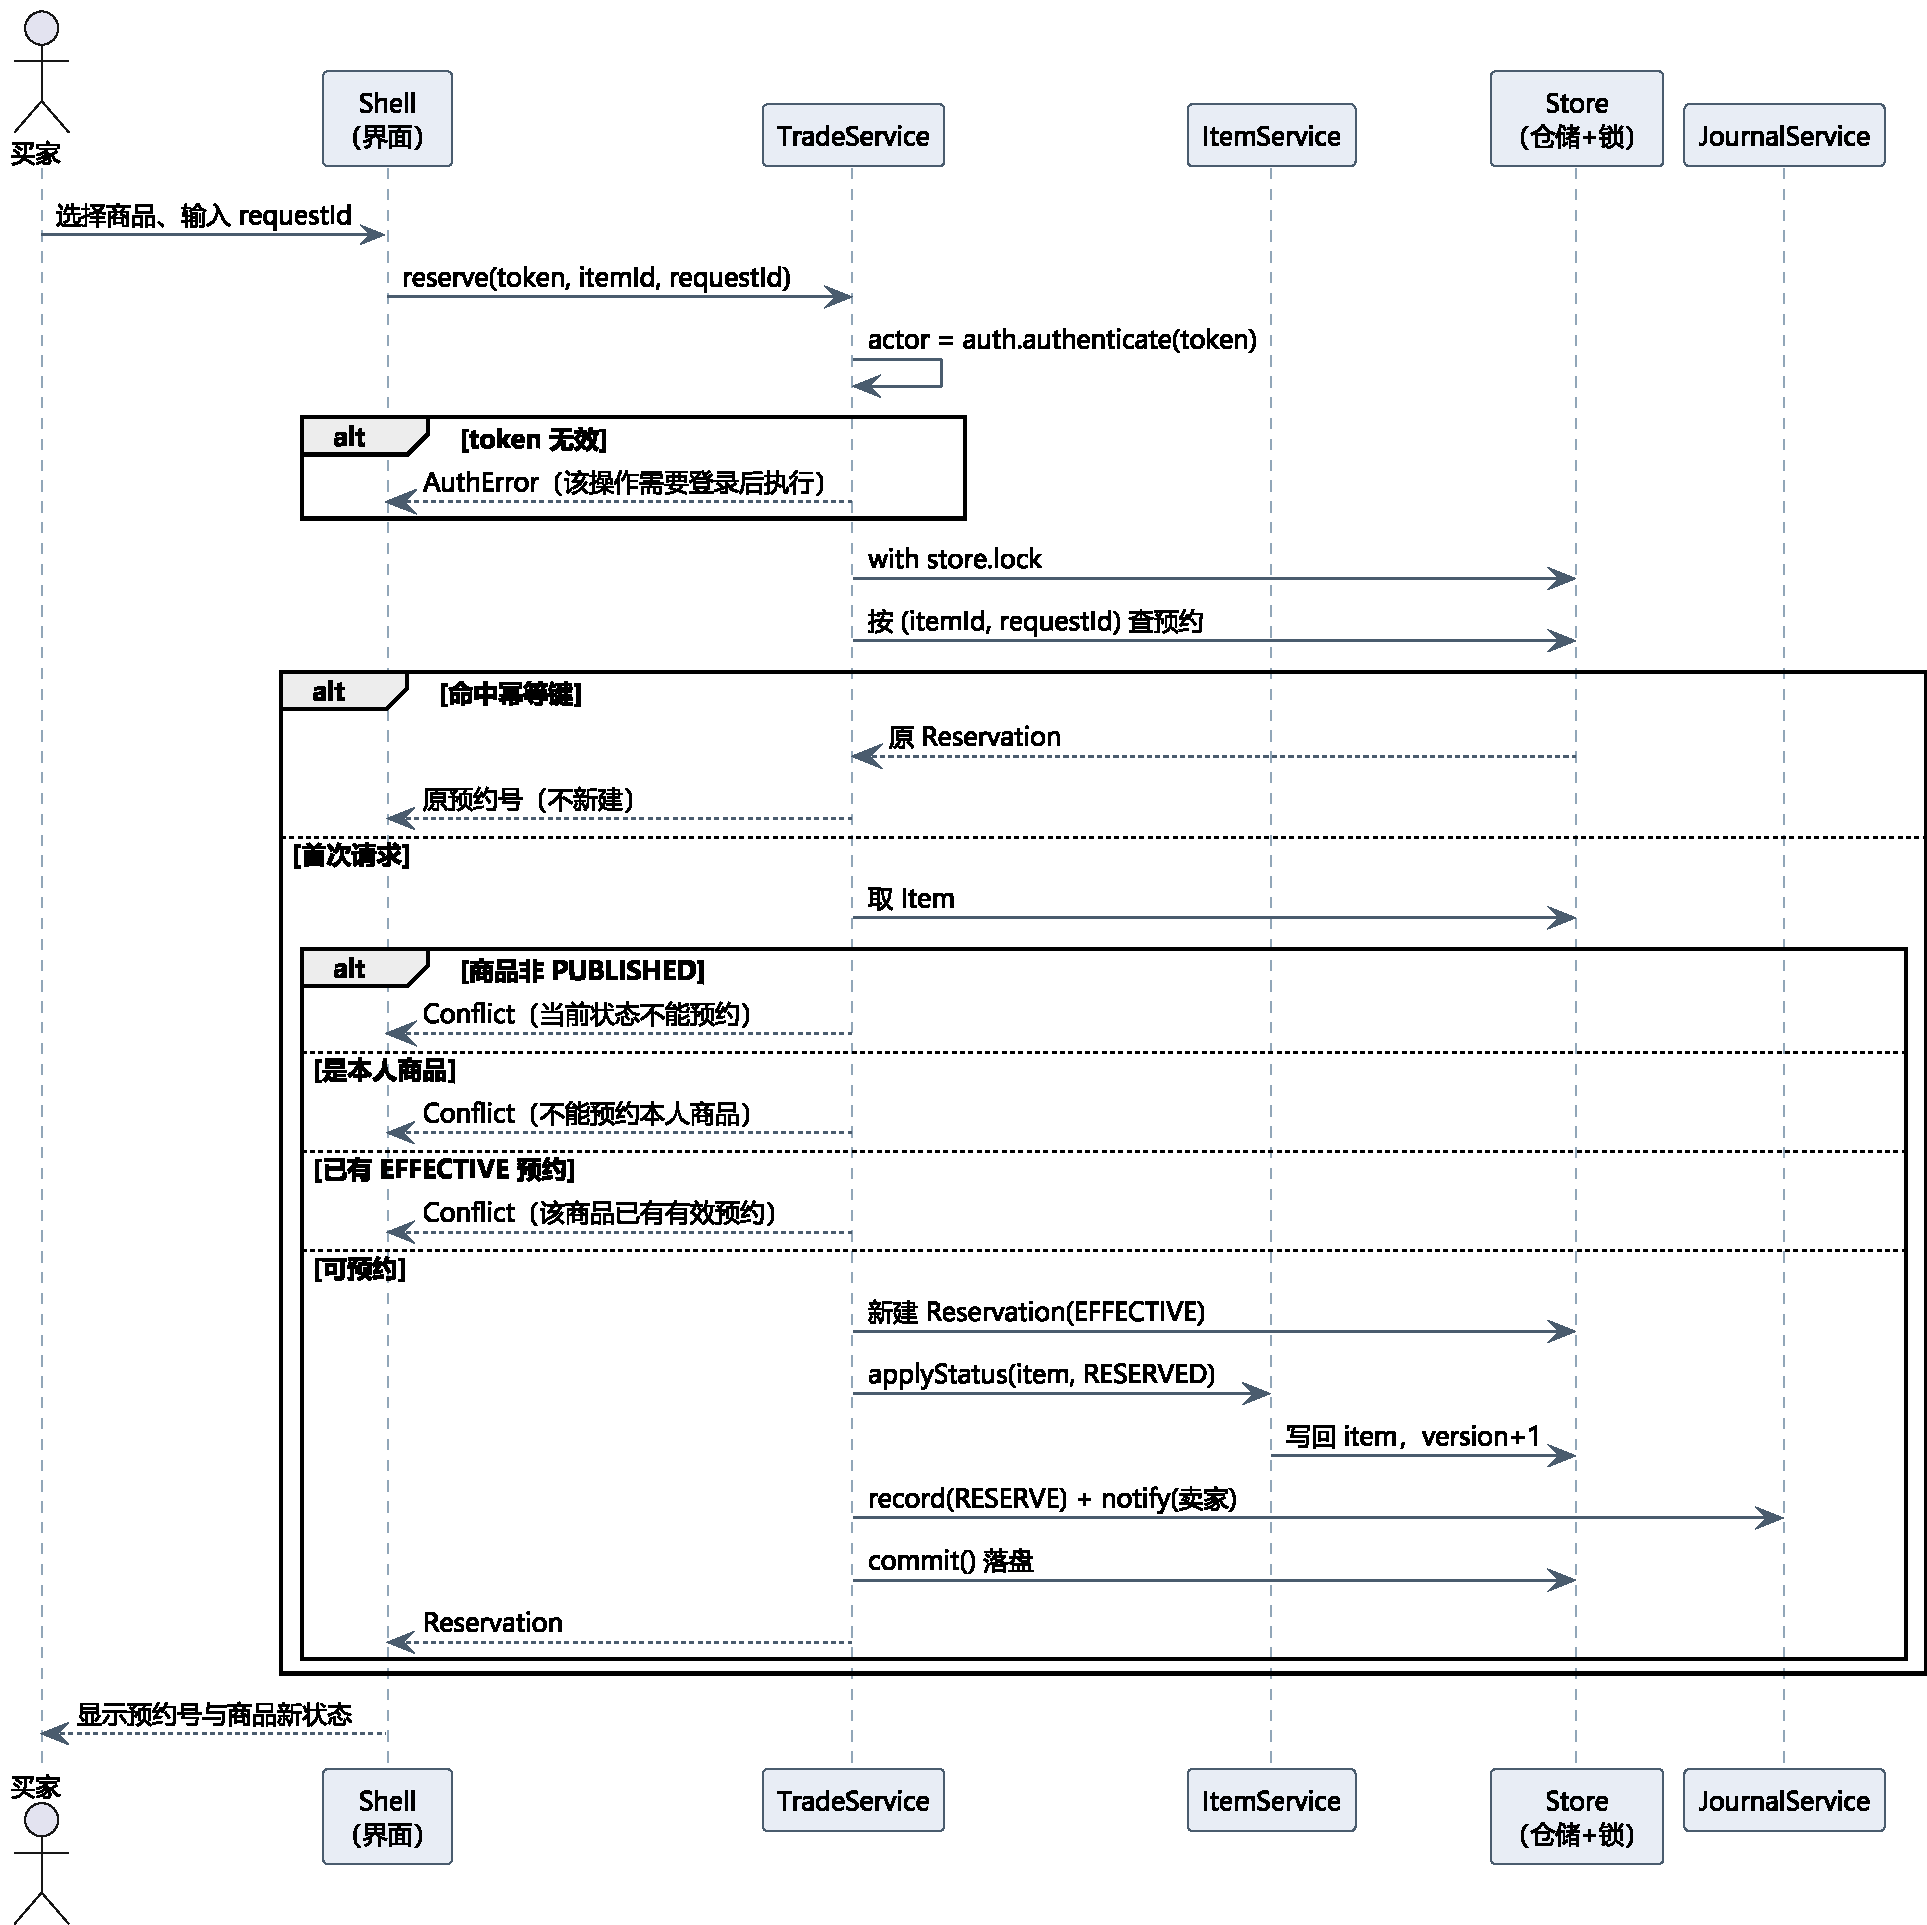
\includegraphics[width=0.74\textwidth]{seq_reserve.pdf}
\caption{预约商品时序图}\label{fig:seq}
\end{figure}

修改已发布商品（\figref{fig:seq2}）把待审内容与商品状态解耦：修改只写 \code{ItemRevision}，前台仍显示旧信息，审核期间买家照常预约；通过时原子替换全部字段，驳回则丢弃待审记录。

\begin{figure}[!htbp]
\centering
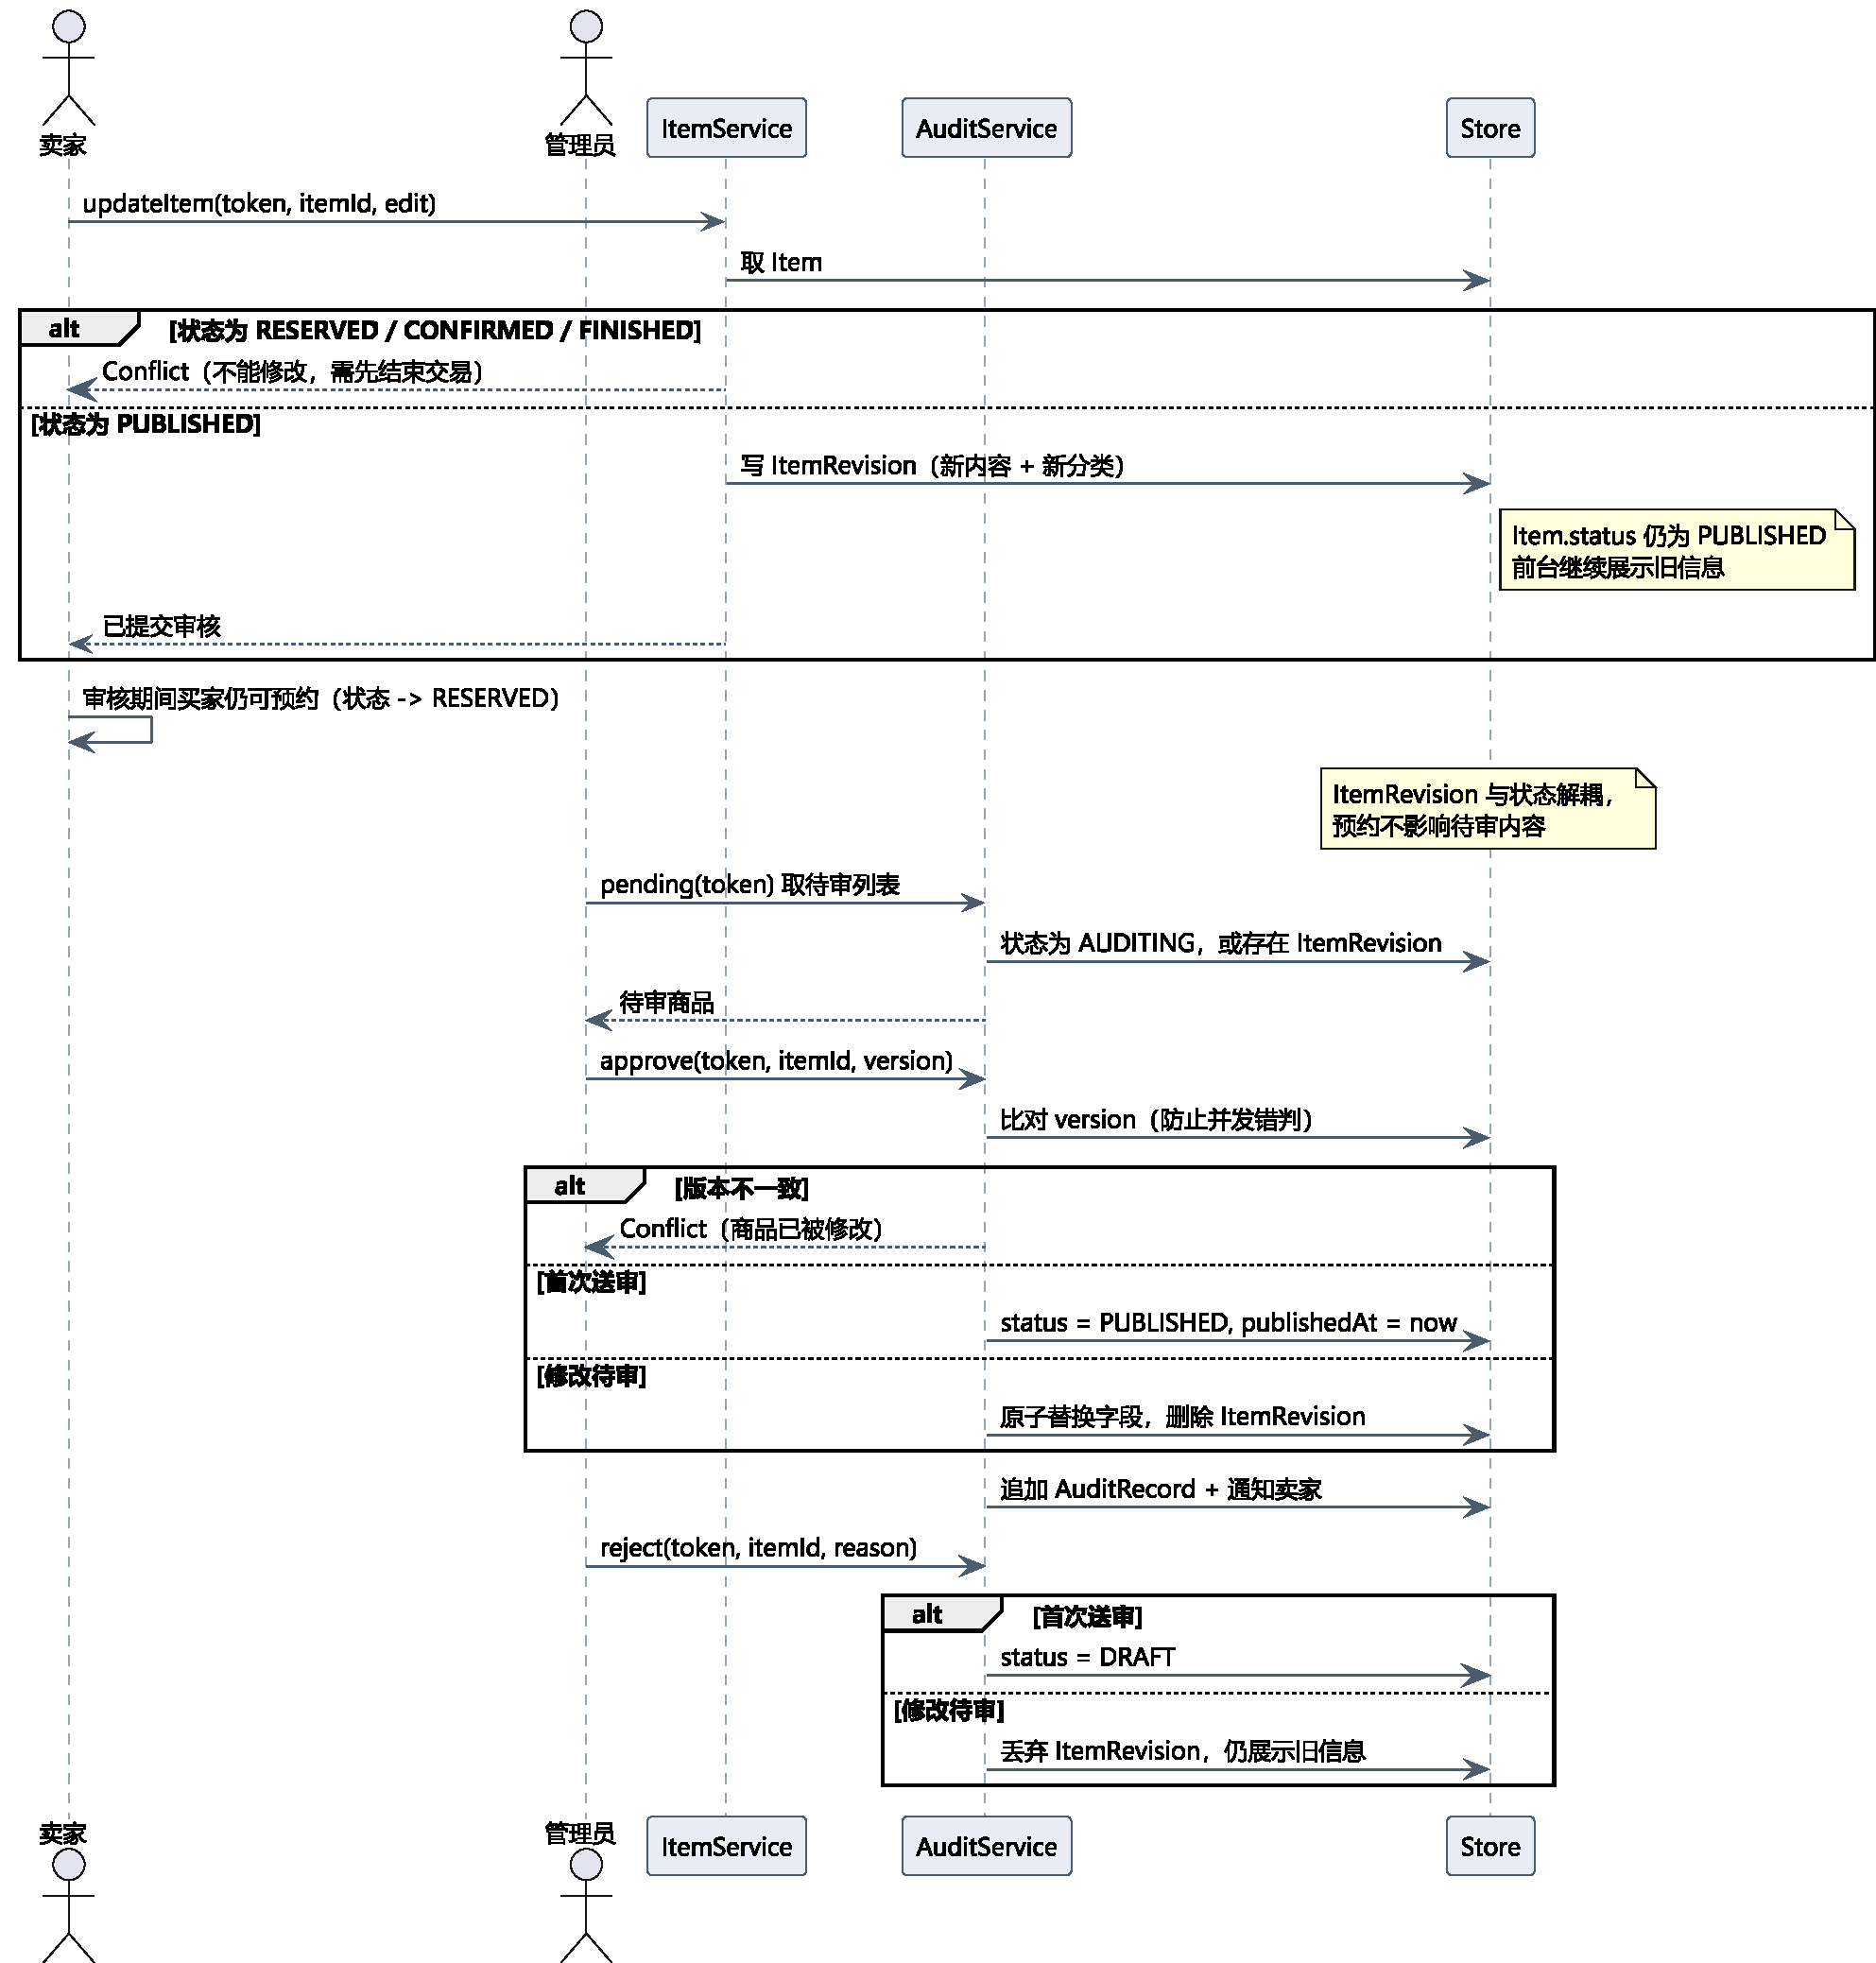
\includegraphics[width=0.7\textwidth]{seq_revision.pdf}
\caption{修改已发布商品与审核时序图}\label{fig:seq2}
\end{figure}

\subsection{代码规模}

共 22 个源文件、3311 行，去掉空行与注释后 \textbf{2761 行}；另有 8 个测试文件、73 个用例（\tabref{tab:loc}）。

\begin{table}[htbp]
\centering
\caption{源代码规模统计}\label{tab:loc}
\zihao{-5}
\renewcommand{\arraystretch}{1.18}
\begin{tabularx}{\textwidth}{@{}L{3.2cm}L{1.6cm}L{2.0cm}L{2.4cm}Y@{}}
\toprule
分组 & 文件数 & 总行数 & 有效代码行 & 主要文件 \\
\midrule
领域模型 & 3 & 513 & 377 & \code{models.py}（327） \\
基础设施 & 2 & 305 & 254 & \code{storage.py}（260） \\
服务层 & 9 & 1343 & 1186 & \code{item.py}（386）、\code{trade.py}（253） \\
界面层 & 3 & 602 & 500 & \code{shell.py}（530） \\
装配与入口 & 5 & 548 & 444 & \code{demo.py}（344） \\
\midrule
小计 & 22 & 3311 & \textbf{2761} & 平均每文件 126 行 \\
测试 & 8 & 794 & 577 & 73 个用例 \\
\bottomrule
\end{tabularx}
\end{table}

\section{大模型辅助开发}

\subsection{使用方式}

直接让模型"照着类图把系统写出来"是我最先排除的做法：需求有 19 条、状态有 7 个，一次生成几百行代码，我既没法逐行核对，也说不清哪条规则由哪段代码保证，出错时只能整段重写。实际采用的是"按模块切分、先规约后实现、每轮跑检查"的方式，共十轮：

\begin{enumerate}[leftmargin=1.6em,itemsep=2pt,topsep=3pt]
\item \textbf{一轮只喂一个模块}。输入是相关的 2--3 条需求原文、类图里对应的那一段 \mbox{PlantUML}、以及已经定下来的接口签名。模块小到能在一屏里核对，错了也只错这一块。
\item \textbf{先要存根与规约，再要实现}。让它先写出方法签名、参数含义、前置条件、后置条件、会抛哪些异常，我确认规约对了再让它填函数体。规约写错的概率远低于实现写错，而且在规约阶段就能发现需求理解偏差。
\item \textbf{每轮结束立刻跑三项检查}。\code{python -m compileall}（语法）、\code{pylint}（风格）、\code{pytest}（行为），把报错原文原样贴回下一轮，让它按报错改，而不是我手工描述错误。
\item \textbf{所有产出都过一遍手}。模型给的每一行我都读过，改动与理由写进 git 提交说明，能对得上"哪一行是模型写的、哪一行是我改的"。
\end{enumerate}

十轮的具体输入、产出与人工处理见\tabref{tab:rounds}，完整记录（含被退回的版本）在仓库 \code{code/docs/prompts.md}。

\begin{table}[htbp]
\centering
\caption{与大模型的十轮交互摘要}\label{tab:rounds}
\zihao{-5}
\renewcommand{\arraystretch}{1.16}
\begin{tabularx}{\textwidth}{@{}L{0.9cm}L{3.6cm}L{4.4cm}Y@{}}
\toprule
轮次 & 输入 & 模型产出 & 人工处理 \\
\midrule
R1 & 19 条需求 + 类图，只做数据模型 & 10 个 dataclass、5 个枚举、异常层次 & 采纳；补 \code{publishedAt}、\allowbreak \code{disputed} 两个字段 \\
R2 & 仓储要能落盘、支持泛型表 & \code{Table}、\allowbreak \code{Store}、\allowbreak 编解码 & 换掉 \code{asdict}（Decimal/datetime 会丢类型），改原子写 \\
R3 & 状态图 puml & 迁移表 + \code{apply\_status} & 采纳；补中文状态名映射 \\
R4 & REQ-002/005/009/014/017 & 商品服务 & \textbf{退回}：初稿直接改已发布商品的字段，改为写待审记录 \\
R5 & REQ-003/019 & 审核服务与审核记录 & 采纳；补版本号比对 \\
R6 & REQ-001/006/007/008/015 & 交易服务 & \textbf{退回}：初稿无锁，改为锁内查重建单 \\
R7 & REQ-010/013/018 & 举报、日志、统计 & 采纳；处置改为复用商品下架 \\
R8 & 全部服务 & 演示脚本、命令行菜单、表格排版 & 采纳结构；修 3 处残留与漏传令牌 \\
R9 & pylint 初稿 27 条告警 & 逐条修复方案 & 采纳 25 条，2 条按项目约定处理 \\
R10 & pytest 失败输出 & 定位到"完成只通知卖家" & 采纳，改代码不改测试 \\
\bottomrule
\end{tabularx}
\end{table}

\subsection{大模型实际承担的工作}

回头看，模型真正省时间的是三类活：

\begin{itemize}[leftmargin=1.6em,itemsep=2pt,topsep=3pt]
\item \textbf{模板化代码}：10 个 dataclass 的字段声明、21 个文件的 \code{\_\_init\_\_}、\allowbreak 异常类层次、\code{argparse} 参数定义。这些没有设计含量，但手打容易漏。
\item \textbf{把图翻成表}：状态图的 9 条箭头、时序图的 \code{alt} 分支，让它逐条列出"箭头 $\to$ 触发方法 $\to$ 抛什么异常"，我再核对是否有漏。我在这一项上最容易看走眼，它不容易。
\item \textbf{检查与修复}：把 pylint 的 27 条告警贴回去，让它给逐条修复方案（折行、改 \code{types.NoneType}、\allowbreak 把多 return 改成单一出口），比我自己一条条查文档快。
\end{itemize}

而设计判断类的活它给不出可靠答案：锁加在哪里、要不要把方法从实体上移走、驳回后商品回不回草稿，这些必须我自己定。它的默认倾向是"能跑就行"，例如初稿愿意让已发布商品的修改直接覆盖字段——功能上似乎也对，但违反了 REQ-017 的展示语义。

\subsection{模型生成不符合预期的四个案例}

\textbf{案例 1：审核服务漏掉"审核期间被预约"的状态。}演示脚本执行到第 7 节时抛 \code{Conflict: 商品当前为已预约，不在待审核状态}。原因是模型按"审核只发生在待审核或已发布"写分支：

\begin{lstlisting}
# 模型初稿：只认两种状态
if item.status is ItemStatus.AUDITING:
    apply_status(item, ItemStatus.PUBLISHED)
elif item.status is ItemStatus.PUBLISHED and revision is not None:
    self._apply_revision(item, revision, now)
else:
    raise Conflict("不在待审核状态")

# 修改后：把"可挂待审内容的状态"抽成常量，三处共用
_REVISION_HOLDERS = (ItemStatus.PUBLISHED, ItemStatus.RESERVED,
                     ItemStatus.CONFIRMED)
elif revision is not None and item.status in _REVISION_HOLDERS:
    self._apply_revision(item, revision, now)
\end{lstlisting}

REQ-017 明确写了"修改审核期间买家仍可预约"，商品会变成已预约，此时待审内容仍应能通过。这个漏洞不是笔误，是模型没有把两条需求交叉起来想。我补了 \code{test\_revision\_can\_be\_approved\_after\_reservation} 用例把它钉住。

\textbf{案例 2：交易完成只通知卖家。}\code{test\_auto\_finish\_after\_seven\_days} 失败，买家收件箱里没有完成通知。REQ-015 原文是"自动将交易标记为已完成\textbf{并通知买家}"，模型把"完成"当成卖家关心的事。判断是测试对、代码错，于是改 \code{\_finish} 同时给买卖双方发通知，测试一行没动。

\textbf{案例 3：把必填校验放在建草稿时。}需求要求"草稿保存成功"与"必填字段缺失时不能提交"两条同时成立，初稿在 \code{create\_draft} 就强制描述非空，导致写了一半的草稿存不下来。改成 \code{\_validate\_fields(draft, strict)} 两档：建草稿只校验标题、价格、分类，提交审核时再查描述。

\textbf{案例 4：编解码函数被 pylint 判为 \code{too-many-return-statements}。}模型的修法是加 \code{\# pylint: disable}，我没有接受，改成"先解 Optional，再按分支给 \code{result} 赋值"的单一出口写法。告警消失的原因是代码真的变简单了，而不是检查被关掉了。

\subsection{我的判断}

有三类产出我明确拒绝了：一是把业务规则塞回实体方法的版本（规则会散落，事务边界不清，见 2.3 节）；二是用 \code{disable} 消警告的版本；三是"先查再写"不加锁的并发实现（在 4 核机器上跑 4 个线程预约同一商品，初稿会建出两条有效预约）。

判断模型输出对不对，我用的是"造反例"：每条它声称的规则，都在演示脚本或测试里造一个应该被拒绝的场景去撞它，撞不穿才算数。上面四个案例全是撞出来的，四个都不在它主动说明的风险里。这也是本次实验最大的收获——模型给的是"看起来对"的代码，验证的成本必须由我自己承担。

\section{代码风格与静态检查}

用 \code{pylint} 4.1.3 做静态检查，标准取 PEP 8（行宽 79、4 空格缩进），配置文件 \code{pylintrc} 放在代码根目录。只关掉三类与作业场景无关的检查：\code{duplicate-code}（模板化的 dataclass 声明必然相似）、\code{too-few-public-methods}（实体本来就只有数据）、\code{too-many-lines}。参数上限放宽到 6 个、属性上限 14 个，因为 \code{Item} 有 13 个字段，这是领域模型本身的样子，拆开反而难读。

第一版可运行代码（不含测试）跑出 \textbf{9.85/10}，共 27 条告警，分布见\tabref{tab:pylintinit}。没有一条是逻辑错误类（\code{E} 级）告警，全是格式与写法问题——"能跑"和"好读"确实是两件事。

\begin{table}[htbp]
\centering
\caption{初稿 27 条告警的分布}\label{tab:pylintinit}
\zihao{-5}
\renewcommand{\arraystretch}{1.15}
\begin{tabularx}{\textwidth}{@{}L{5.0cm}L{1.2cm}L{3.6cm}Y@{}}
\toprule
告警 & 条数 & 典型位置 & 处理方式 \\
\midrule
\code{line-too-long} C0301 & 22 & 6 个文件，最长 83 字符 & 按语义折行，不缩排 \\
\code{trailing-newlines} C0305 & 2 & \code{item.py}、\code{moderation.py} & 删除文件末尾多余空行 \\
\code{unidiomatic-typecheck} C0123 & 1 & \code{storage.py:60} & \code{type(None)} 改为 \code{types.NoneType} \\
\code{too-many-return-statements} R0911 & 1 & \code{storage.py:54} & 重写为单一出口 \\
\code{unused-import} W0611 & 1 & \code{auth.py:12} & 删除未使用的 \code{NotFound} \\
\bottomrule
\end{tabularx}
\end{table}

行宽占 22 条，其中 15 条只超 1--4 个字符，删几个空格也能过，但那样只是把问题藏起来。按语义折行才是对的：函数调用的参数对齐到左括号后，\code{if} 的条件用括号包起来再按布尔项分行。

\begin{lstlisting}
# 修复前（83 字符）
self._journal.record(actor.user_id, action, item.item_id, True, item.title)

# 修复后：按"调用参数对齐"折行
self._journal.record(
    actor.user_id, action, item.item_id, True, item.title)
\end{lstlisting}

把测试代码一起纳入检查后重新跑，得分 \textbf{10.00/10}：

\lstinputlisting{listings/pylint_after.tex}

测试目录有三处文件级 \code{disable}，都写了理由：pytest 夹具互相引用是官方写法（\code{redefined-outer-name}）、用例名本身就是文档（\code{missing-function-docstring}）、有的夹具只负责铺数据（\code{unused-argument}）。除此之外没有其它豁免，源码目录一条 \code{disable} 都没有。

这次也吃了晚检查的亏：第一次跑 pylint 是写完 3000 行之后，27 条里 22 条是行宽，属于写的时候就该注意的问题，攒到最后改就是一次几百行的机械劳动。

\section{编译与运行结果}

\subsection{运行环境}

\begin{table}[htbp]
\centering
\caption{运行与检查环境}\label{tab:env}
\zihao{-5}
\renewcommand{\arraystretch}{1.15}
\begin{tabularx}{\textwidth}{@{}L{3.0cm}L{5.0cm}Y@{}}
\toprule
项目 & 版本 / 型号 & 说明 \\
\midrule
操作系统 & Windows 11（win32） & 命令行使用 Git Bash \\
Python & 3.13.14 & 仅标准库；无运行时第三方依赖 \\
代码检查 & pylint 4.1.3 & PEP 8，行宽 79 \\
单元测试 & pytest 9.2.0 & 73 个用例 \\
UML 渲染 & PlantUML 1.2024.8 + OpenJDK 17 & 输出 190 dpi PNG \\
报告排版 & TeX Live 2025（XeLaTeX + ctex） & —— \\
\bottomrule
\end{tabularx}
\end{table}

\subsection{编译检查}

Python 是解释型语言，没有独立的编译步骤；为满足"使用编译器或 IDE 编译"的要求，用标准库 \code{compileall} 对全部源码做字节码编译，它会同时暴露语法错误与模块导入错误：

\begin{lstlisting}
$ python -m compileall -q campustrade run.py tests
$ echo $?
0
\end{lstlisting}

没有任何输出、退出码为 0，说明 22 个源文件与 8 个测试文件都能通过语法与导入检查。运行时验证由 \code{python run.py --demo}（端到端）与交互式 \code{python run.py --seed} 两条路径覆盖，下面分别给出真实输出。

\subsection{单元测试}

\begin{lstlisting}
$ python -m pytest -q
\end{lstlisting}

\lstinputlisting{listings/pytest.tex}

测试按模块分文件，覆盖关系见\tabref{tab:tests}。这里刻意没有追求行覆盖率数字，而是每写一条规则就配一个"应该被拒绝"的用例：权限越权、状态不允许、重复提交、时间未到，这些分支才是真实缺陷的藏身处。

\begin{table}[htbp]
\centering
\caption{测试文件与覆盖的需求}\label{tab:tests}
\zihao{-5}
\renewcommand{\arraystretch}{1.15}
\begin{tabularx}{\textwidth}{@{}L{3.4cm}L{1.4cm}Y@{}}
\toprule
测试文件 & 用例数 & 覆盖内容 \\
\midrule
\code{test\_auth.py} & 12 & 注册、登录、重复学号、弱口令、会话过期、停用账号、改密码（REQ-004/012/016） \\
\code{test\_item.py} & 15 & 草稿、公开查询过滤与排序、必填校验、下架与恢复、分类唯一性与引用保护（REQ-002/005/009/014） \\
\code{test\_audit.py} & 10 & 通过/驳回、待审内容原子替换、驳回丢弃、版本冲突、审核历史与可见性（REQ-003/017/019） \\
\code{test\_trade.py} & 13 & 幂等重发、唯一有效预约、取消、确认、完成、超时自动完成、异议暂停、并发竞争（REQ-001/006/007/008/015） \\
\code{test\_moderation.py} & 8 & 举报去重、处置下架/驳回、重复处理、已预约商品不能下架（REQ-010/014） \\
\code{test\_storage.py} & 10 & JSON 快照往返（Decimal/枚举/时间）、时间范围统计、日志权限、损坏文件处理（REQ-013/018） \\
\code{test\_cli.py} & 5 & 登录、搜索、预约、非法选项、管理员菜单的界面冒烟 \\
\midrule
合计 & 73 & —— \\
\bottomrule
\end{tabularx}
\end{table}

\subsection{端到端演示}

\code{python run.py --demo} 在内存库上按需求编号跑 11 节场景，每节既有"应当成功"的路径，也有"应当被拒绝"的反例，最后打印是否出现未捕获异常。完整输出如下（\code{√} 表示按预期成功，\code{×} 表示按预期被拒绝）：

\lstinputlisting{listings/demo.tex}

几个值得单独说明的结果：

\begin{itemize}[leftmargin=1.6em,itemsep=2pt,topsep=3pt]
\item 第 4 节：同一 \code{requestId} 重发返回预约号 1，预约记录仍只有 1 条，"重发不算新请求"落地；另一买家再预约被拒，唯一性成立。
\item 第 7 节：修改已发布商品后前台仍显示《罗技 M590 静音鼠标》89 元，期间买家仍能预约（预约号 3），审核通过后价格变为 79 元且待审记录被清除；驳回的那一件仍显示原价 45 元。
\item 第 9 节：4 个买家经屏障同步后同时预约，只有 1 个成功，其余 3 个收到 \code{CONFLICT}。商品最终只有 1 条有效预约。
\item 第 10 节：把确认时间回拨 8 天后触发自动完成，商品变已完成，卖家与买家都收到通知。
\end{itemize}

\subsection{交互式运行}

\code{python run.py --seed} 进入菜单界面，下面是真实会话。为节省篇幅，省去了每条命令后重复打印的菜单与输入提示，只在 \code{→} 后保留该步的执行结果，其余原样保留：管理员审核通过一件待审商品，买家搜索并预约，卖家确认交易，买家确认完成，最后卖家查看统计。

\lstinputlisting{listings/cli.tex}

会话中可以看到权限是按身份变化的：管理员登录后菜单多出 21--30 项（审核、举报、统计、日志、分类），普通用户只有 1--15 项；未登录时只能浏览商品。最后一行"发布 4 件，预约 1 次，完成 1 笔，交易额 45.00 元"与前面几步的操作完全对得上，说明统计口径没有把别人的数据算进来。

\section{Git 远程代码管理}

本地仓库在 \code{repo/}，远程托管在 GitHub：

\begin{lstlisting}
$ git remote -v
origin  https://github.com/APY-tech/Software-Engineering.git (fetch)
origin  https://github.com/APY-tech/Software-Engineering.git (push)
\end{lstlisting}

主分支 \code{main}，三次实验的产物都在同一仓库里，靠目录与提交说明区分，没有另开分支——交付物是持续演进的同一个项目，分支反而增加合并成本。实验一的两次关键状态另打了标签 \code{lab1-ai-draft} 与 \code{lab1-final}，便于对照初稿与定稿。

本轮工作按"一类产物一次提交"拆开（\tabref{tab:commits}）：代码与它的检查记录分开，报告单独提交，避免 3000 行代码和一份 PDF 混在一个提交里导致 diff 无法阅读。

\begin{table}[htbp]
\centering
\caption{本次实验的提交记录}\label{tab:commits}
\zihao{-5}
\renewcommand{\arraystretch}{1.15}
\begin{tabularx}{\textwidth}{@{}L{1.8cm}L{1.5cm}Y@{}}
\toprule
提交 & 文件数 & 内容 \\
\midrule
\code{a66e16a} & 34 & 22 个源文件、8 个测试文件、配置与说明 \\
\code{31056f2} & 8 & pylint 前后对比、测试与演示输出、代码规模、提示词记录 \\
\code{ad62b25} & 12 & 类图、服务类图、两张时序图的 puml 与 png \\
\code{e2e555f} & 20 & 报告 LaTeX 源、插图与编译产物 \\
\bottomrule
\end{tabularx}
\end{table}

仓库最新的提交历史：

\lstinputlisting{listings/git.tex}

\code{.gitignore} 排除了三类东西：Python 的 \code{\_\_pycache\_\_/} 与 \code{.pytest\_cache/}；程序运行产生的 \code{code/data/campustrade.json}（可用 \code{--seed} 重建，不占仓库体积）；LaTeX 中间产物（\code{.aux}、\code{.log}、\code{.toc}）。源码、UML 的 puml 与图、测试、检查记录、报告源与 PDF 都入库。


\end{document}
